\chapter{引言}\label{chap:one}

\section{研究背景}


随着互联网技术的不断发展,网民规模继续保持平稳增长,根据 CNNIC 发 布的《第 41 次中国互联网发展状况统计报告》显示\citep{CNNIC},截止 2017 年 12 月,我 国网民达到 7.72 亿,全年共计新增网民 4074 万人,互联网普及率达到 55.8\%, 增长率达到 2.6\%,如图1.1所示。与此同时互联网模式不断创新,互联网上出现 了众多的社交媒体,比如微博、Twitter、微信、博客、论坛、社交网站等。社交 媒体的出现彻底改变了人们获取信息和传播信息的方式\citep{wuyue1}。


\begin{figure}[!htbp]
    \centering
    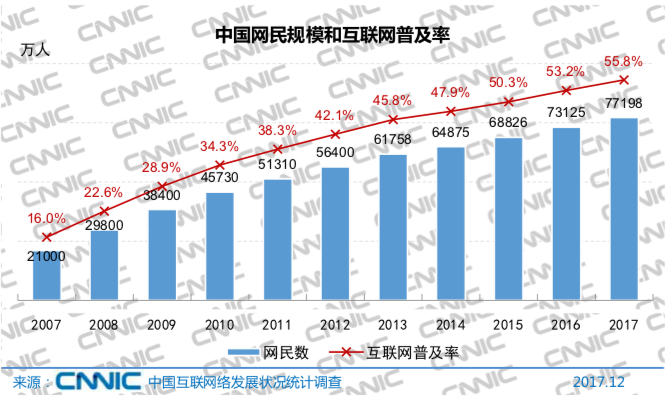
\includegraphics[width=0.8\textwidth]{1-1-1}
    \bicaption{中国网民规模和互联网普及率\citep{CNNIC}}{Chinese Internet users scale and Internet penetration rate\citep{CNNIC}}
    \label{fig:1-1-1}
\end{figure}

在不同形式的社交媒体中,微博以其独特的社交方式、巨大的网民基础和多 媒体技术之间的融合,成为当今信息产生和传播的重要平台。随着网民规模的不 断扩大,使用社交网络的用户也呈现出爆发增长的态势,微博用户逐年增加,覆 盖的群体越来越广,微博月活跃用户如图\ref{fig:a}所示。微博平台的用户不仅是信息 的接受者,同时可以是信息的产生者和传播者。这种“去中心化”的信息传播模式 使得信息可以在短时间内迅速在社交网络上广泛传播,从而产生巨大的社会影 响。

\begin{figure}[H]
    \centering
    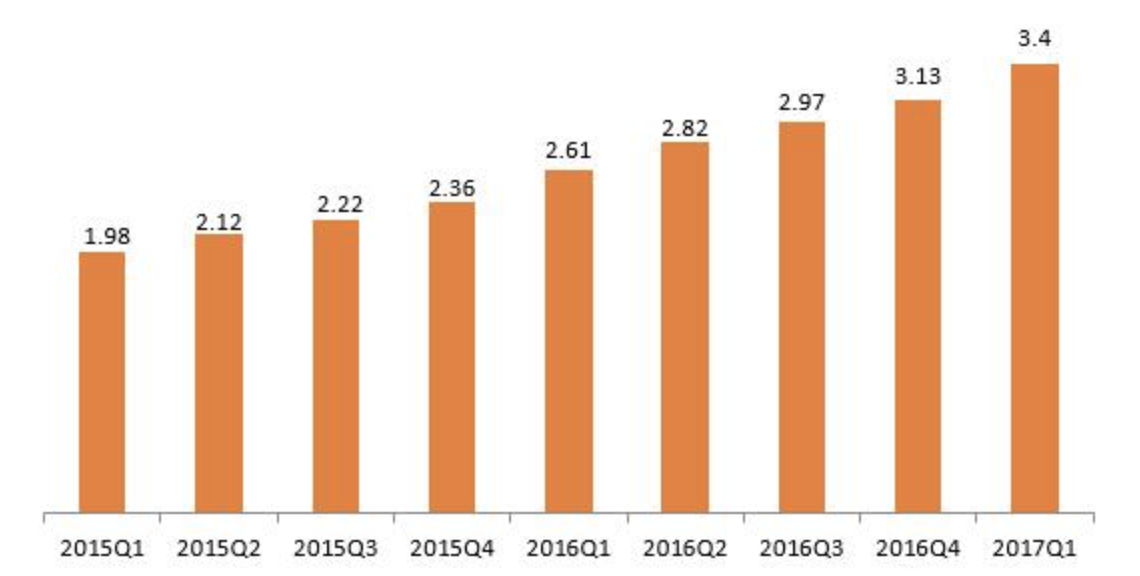
\includegraphics[width=0.6\textwidth]{a}
    \bicaption{微博月活跃用户\citep{weibo}}{Microblogging monthly active users\citep{weibo}}
    \label{fig:a}
\end{figure}


微博等社交应用的出现极大地降低了社会网络中用户间信息交流的成本,大 量用户通过社交网络积极地参与信息传播,使得社交平台上的信息传播呈现出 传播速度快、覆盖范围广和社会影响力深等特点;在传播范围上,社交信息的传 播还具有流行度呈现幂律分布的特点 \citep{Bakshy2011Everyone},即仅有少部分信息能够被大量用户转 发,而大部分信息只有很少的人会关注,不会变得流行。产生这种现象的主要原 因是社会网络中的信息存在过载问题,使得用户注意力成为稀缺资源 \citep{Davenport2001The},信息 只有在引起足够多用户关注的前提下才能够生存并继续传播。

微博作为社会交流和信息传播的主要平台之一,已经成为国内网络用户的 主要信息来源。在微博的消息传播中常出现消息的阵发性现象,即一个讨论的话 题的产生到流行,会在一个短时间内发生,然后很快就会消失。这样的突发话题 通常是由突发新闻、真实事件、恶意谣言或各种各样的行为引发的。这些爆炸性 的话题,通常被称为热门话题,为用户提供最新的事件。因此预测热门话题在很 多方面至关重要,如销售、股票市场、搜索引擎查询、选举,甚至是疾病爆发。 因此,更早的发现这些突发事件意味着增加收入,减少损失,及时治疗,以及更 好的决策。但同时由于这种话题的阵发性,导致了阵发话题的预测存在相当的困 难。

在微博和 Twitter 中,主题标签通常以 Hashtag 作为标识\citep{shaojian2}。在微博或是 Twitter 用户发送的消息中,带有以 \# 开头和结尾的文字即便认为该消息带有主 题标签,各种主流微博平台都提供了 Hashtag 标注功能,如关于马航坠机事件的 Hashtag 在 Twitter 中为“\#MH370”,在新浪微博中为“\#MH370\#”。虽然不同平台 中 Hashtag 的具体标记形式可能不同,但功能基本相同,都具有主题标注和话题 参与的功能。主题标注功能指 Hashtag 能够表达一条微博中的主题信息,话题参 与功能指用户使用 Hashtag 参与同一个话题的讨论。在微博平台中,上述功能使Hashtag 在信息组织和信息检索方面具有优势,因此越来越多的学者开始深入研究 Hashtag。


\section{研究意义}

根据从微博的数据中分析得到,我们每天可以识别数十万个新 Hashtag。 Hashtag 作为一个用户自发打下的标签,表达了用户真实想法,对于捕捉用户 兴趣和关注有极大作用。并且在微博上 Hashtag 的流行度反映了当下的社会群体 的关注点,表述了网民对于事件的重视程度。如图\ref{fig:b}所述,十九大期间,“\# 十九 大 \#”这个 Hashtag 出现了几十亿次,直观的反映了人们对于该事件的关注程度。 因此 Hashtag 在突发事件监测 \citep{Hughes2009Twitter}、流行电视节目评论监测 \citep{Deller2011Twittering} 和公众对政府的态 度监测 \citep{small2011hashtag}等方面发挥重要的作用。本文从微博的实际场景出发,根据 Hashtag 的自身特性进行相关研究,构建 Hashtag 的流行度预测,关注其未来趋势,对于 发现热门话题十分重要。

\begin{figure}[!htbp]
    \centering
    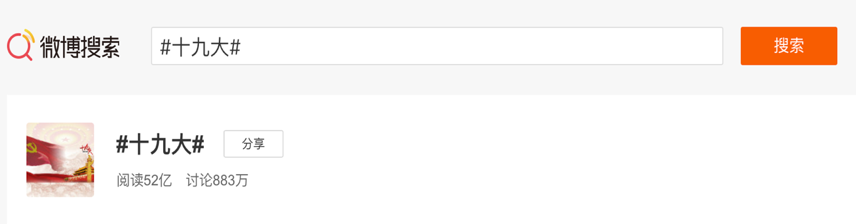
\includegraphics[width=0.8\textwidth]{b}
    \bicaption{Hashtag 热度展示}{Hashtag heat display}
    \label{fig:b}
\end{figure}

\section{面临的问题和挑战}
结合上述背景,本文的任务为 Hashtag 流行度预测,并将其应用在事件流行 度预测模型中,所面临的主要问题和挑战有以下两点:
\begin{enumerate}
\item 现有的社交网络的 Hashtag 流行度预测问题没有考虑用户之间的社交网 络结构特征以及 Hashtag 自身的特性。当前的流行度预测问题,主要考虑的 Hash- tag 的时间序列特征以及 Hashtag 的内容特征,例如考虑时间间隔内 Hashtag 的 转发次数,来预测接下来的转发情况,当然时间序列特征是一个直观并且比较有 效的特征,它很好的反映了消息一个时间段的热门程度。但是 Hashtag 本身是由 用户产生并且进行转发的,用户之间的关注关系是十分重要。并且 Hashtag 有其 自身特性,比如情感性,地域性以及事件性,这些都是其自身重要的特征,对于 预测 Hashtag 的流行度具有很大作用。因此,本文希望在现有的特征的基础上考虑用户的网络结构特征以及 Hashtag 的自身特性,更好的进行 Hashtag 流行度预 测。
\item 传统的消息流行度预测都是单源问题,即消息都是由一个个体发出然后 进行转发传播,但是相同的 Hashtag 可以由不同的个体从不同的时刻发出,如何 处理多源 Hashtag 是本文面临的一大挑战。本文希望通过给出合适的 Hashtag 流 行度预测模型,更好地处理多源消息的预测问题。
\end{enumerate}

\section{论文的研究内容}
本文以面向主题标签流行度预测为研究主体,并实现与之对应的事件流行
度预测框架。针对 1.3 中涉及的问题,本文的研究内容将主要包括以下三个方面:
\begin{enumerate}
\item 在传统的基于特征的 Hashtag 流行度预测的基础上结合用户社交网络结 构信息以及 Hashtag 自身特性,进行更加全面的流行度预测算法。
\item 从消息单源特性出发,考虑 Hashtag 的多源性,结合 Hashtag 传播过程中 的时间因素,实现基于多源头的 Hashtag 流行度预测算法。

\item 整合基于特征的 Hashtag 流行度预测算法,考虑性能以及用户群体等信 息,实现完整的具有较高预测性能的事件热度预测框架。
\end{enumerate}


\section{论文的贡献}
基于 1.4 中的研究内容,本文的贡献主要有以下几点:
\begin{enumerate}
\item 从Hashtag自身特性以及用户粉丝的网络结构特性出发,对已有的微博文 本以及时间序列特征进行扩充,利用用户粉丝的网络结构向量特征,以及 Hashtag 的情感性,地域性,人物性等特征进行模型训练。实验结果表明,新提出来的特 征对于 Hashtag 的流行度预测问题有了一定的效果,也即证明新提出的特征有效 的表达了 Hashtag 的传播特性。
\item 结合外部知识,利用已知的用户粉丝网络结构,提出多源的 Hashtag 流 行度预测模型:利用已知的用户粉丝网络结构,学习用户的向量表达,将其和 Hashtag 的传播路径作为模型的输入进行训练学习,实现用户粉丝网络结构和多 源模型的整合。在大规模微博语料上,对多源 Hashtag 流行度预测模型进行了实 验验证。实验结果表明,模型可以有效地处理多源头的 Hashtag 流行度预测问题。

\item 事件热度预测系统的实现与部署,论文考虑到 Hashtag 可以作为微博中 的事件或者话题,采用基于特征的 Hashtag 流行度预测模型,搭建了事件热度预 测系统。事件热度预测系统通过自动分析微博数据,利用本文提出的主题标签流行度预测算法,进行事件热度预测,通过系统验证了模型的有效性。结果表明,本文提出的事件热度预测具有较高的应用价值。

\end{enumerate}

\section{论文的组织结构}
论文共分为六个章节,主要内容有:

第一章介绍本文的研究背景、研究内容和主要贡献,并给出了本文的组织结 构。

第二章介绍了与本文研究内容相关的流行度预测的相关工作和国内外研究 现状。基于特征的流行度预测方面介绍了现有的流行度预测所考虑到的特征以 及使用的模型;基于消息传播过程的方面分别介绍了点过程以及深度学习方面 的应用。

第三章提出了基于用户网络结构特征以及主题标签自身特性的主题标签流 行度预测算法。从宏观角度出发,不考虑 Hashtag 的传播过程,利用机器学习, 考虑用户粉丝网络结构特征以及 Hashtag 情感性,地域性等特征,采用 xgboost 模型进行 Hashtag 流行度预测;最后通过实验验证模型的有效性。

第四章提出了多源头的主题标签流行度预测。从微观角度出发,考虑 Hashtag 的传播过程,针对 Hashtag 的多源性使用循环神经网络模型,刻画 Hashtag 的传 播过程,结合用户的网络结构特征作为先验知识,进行 Hashtag 流行度预测;最 后通过实验验证模型的有效性。

第五章提出了主题标签流行度预测在事件热度预测系统中的应用。考虑 Hashtag 可以作为微博消息的事件或者话题的特性,采用基于特征的 Hashtag 流 行度预测方法,利用多种组合特征,采用机器学习模型,实现了事件热度预测系 统;最后通过实际应用验证了该模型的有效性和实用性。

  第六章总结了本文中的工作,并对未来研究工作进行了展望。